\section{Modelo de Mezcla Gaussiana} \label{sec_GMM}

Do Chuong y Batzoglou nos indican, en su artículo \textit{What is the expectation maximization algorithm?} [\ref{ChuongBatzoglou}], que el algoritmo de maximización de la esperanza (EM) es una generalización natural de la estimación por máxima verosimilitud. Ésto para el caso en donde se tiene información incompleta.

Los parámetros iniciales se toman de los datos con ello se obtienen unos parámetros finales que se convierten en los parámetros de la siguiente iteración. Así sucesivamente.


\begin{figure}[H]
\centering
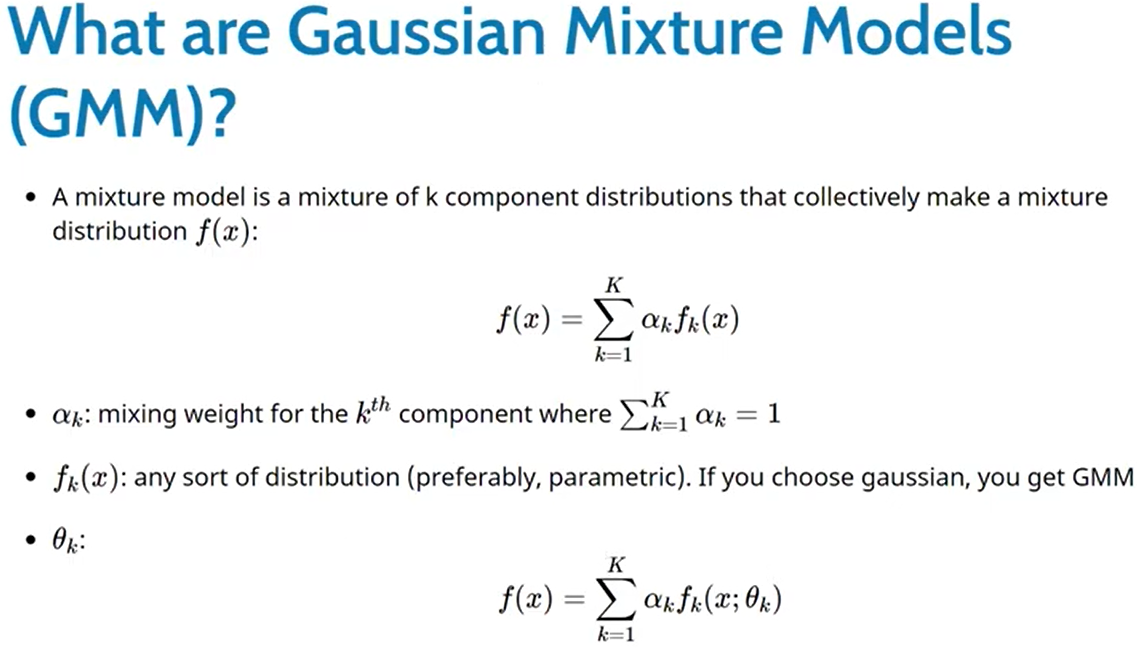
\includegraphics[scale = 0.5]{GMM_1} %width=\textwidth
\caption{\textit{GMM 1}}
\end{figure}

\begin{figure}[H]
\centering
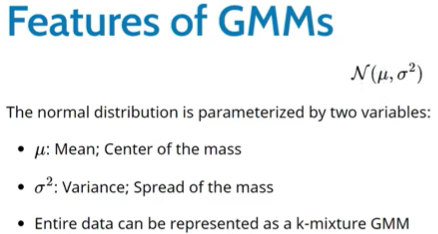
\includegraphics[scale = 0.5]{GMM_2} %width=\textwidth
\caption{\textit{GMM 2}}
\end{figure}

\begin{figure}[H]
\centering
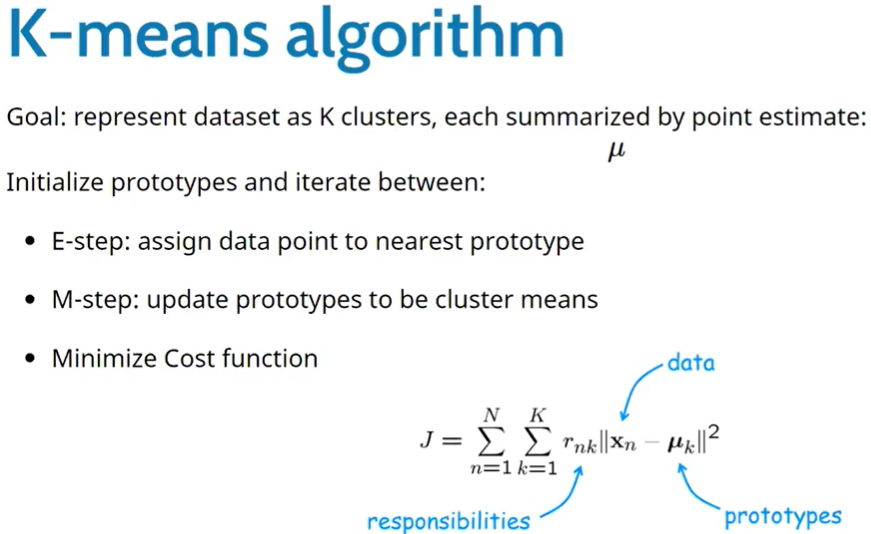
\includegraphics[scale = 0.5]{GMM_3} %width=\textwidth
\caption{\textit{GMM 3}}
\end{figure}

\begin{figure}[H]
\centering
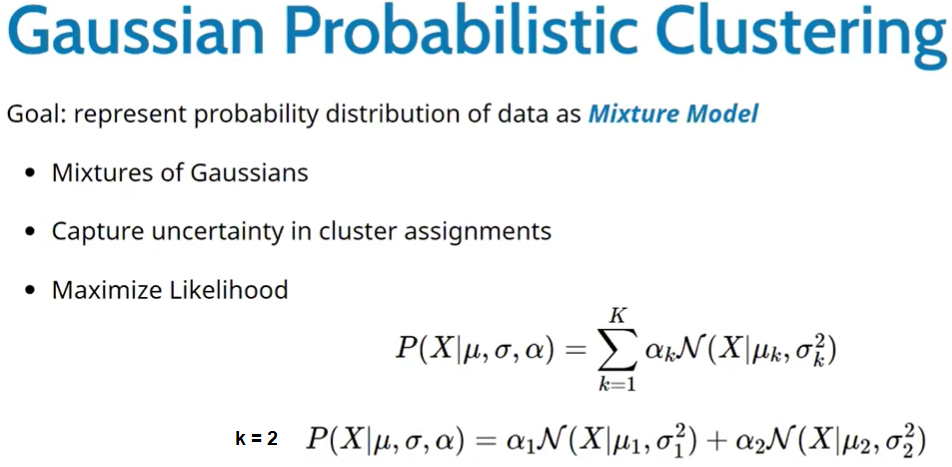
\includegraphics[scale = 0.5]{GMM_4} %width=\textwidth
\caption{\textit{GMM 4}}
\end{figure}

\begin{figure}[H]
\centering
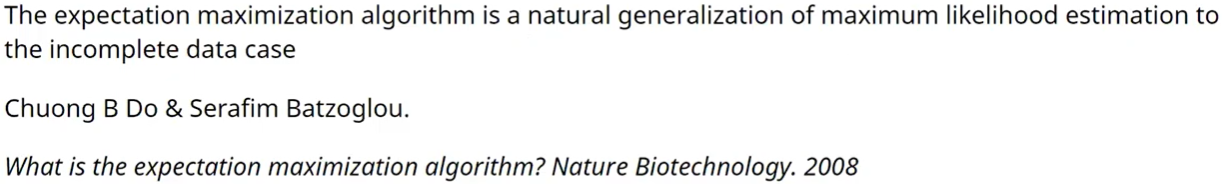
\includegraphics[scale = 0.5]{GMM_5} %width=\textwidth
\caption{\textit{GMM 5}}
\end{figure}

\begin{figure}[H]
\centering
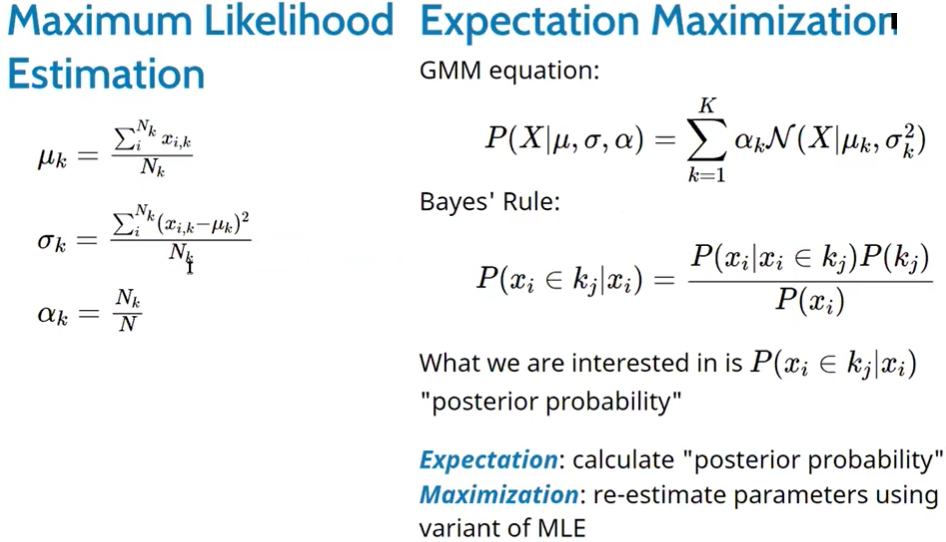
\includegraphics[scale = 0.5]{GMM_6} %width=\textwidth
\caption{\textit{GMM 6}}
\end{figure}

\begin{figure}[H]
\centering
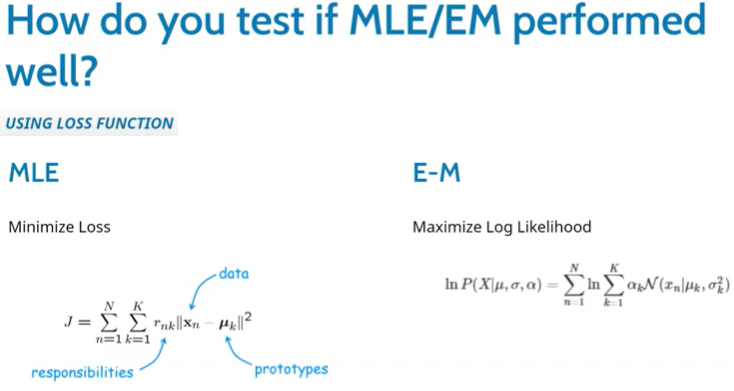
\includegraphics[scale = 0.5]{GMM_7} %width=\textwidth
\caption{\textit{GMM 7}}
\end{figure}
